\documentclass[11pt,twoside]{report}

\usepackage[algoruled]{algorithm2e}
\usepackage{amsfonts}
\usepackage{amsmath}
\usepackage{amssymb}
\usepackage{bm}
\usepackage{cleveref}
\usepackage{color}
\usepackage{fontspec}
\usepackage{mathpazo}
\usepackage{mathtools}
\usepackage{minted}
\usepackage{wrapfig}
\usepackage[separate-uncertainty=true]{siunitx}

\usepackage[intoc, english]{nomencl}
\makenomenclature

\setmonofont[Mapping=tex-text]{Menlo}
\usemintedstyle{}

% This is for writing only, so it's easier to read.
\usepackage[paperheight=9.12in,paperwidth=6.389in,tmargin=.4in,bmargin=.6in,inner=.2in,outer=.4in,heightrounded]{geometry}

\renewcommand*{\thefootnote}{[\arabic{footnote}]}

\allowdisplaybreaks

%\setmainfont{Palatino Linotype}
% The Palatino package gives a pretty terrible look to the PDF when compiling on
% Windows, so we need to use fontspec instead. Palatino Linotype exists on
% Windows but not on Mac (where Palatino exists instead). So...
\suppressfontnotfounderror1
\def\myfont{Palatino}
\def\myfallback{Palatino Linotype}
\count255=\interactionmode
\batchmode
\font\foo="\myfont"\space at 10pt
\ifx\foo\nullfont
  \font\foo = "\myfallback"\space at 10pt
  \ifx\foo\nullfont
    \errorstopmodep
    \errmessage{no suitable font found}
  \else
    \let\myfont=\myfallback
  \fi
\fi
\interactionmode=\count255
\setmainfont[Ligatures=TeX]{\myfont}

% This will add the units
%----------------------------------------------
\newcommand{\nomunit}[1]{%
\renewcommand{\nomentryend}{\hspace*{\fill}#1}}
%----------------------------------------------


\DeclareSIUnit{\parsec}{pc}

% Define common symbols
\newcommand\bphi{\bm{\phi}}
\newcommand\bvarphi{\bm{\varphi}}
\newcommand\bbE{\mathbb{E}}
\newcommand\bbN{\mathbb{N}}
\newcommand\bbR{\mathbb{R}}

\newcommand\bA{\mathbf{A}}
\newcommand\bB{\mathbf{B}}
\newcommand\bC{\mathbf{C}}
\newcommand\bD{\mathbf{D}}
\newcommand\bE{\mathbf{E}}
\newcommand\bF{\mathbf{F}}
\newcommand\bG{\mathbf{G}}
\newcommand\bH{\mathbf{H}}
\newcommand\bI{\mathbf{I}}
\newcommand\bJ{\mathbf{J}}
\newcommand\bK{\mathbf{K}}
\newcommand\bL{\mathbf{L}}
\newcommand\bM{\mathbf{M}}
\newcommand\bN{\mathbf{N}}
\newcommand\bO{\mathbf{O}}
\newcommand\bP{\mathbf{P}}
\newcommand\bQ{\mathbf{Q}}
\newcommand\bR{\mathbf{R}}
\newcommand\bS{\mathbf{S}}
\newcommand\bT{\mathbf{T}}
\newcommand\bU{\mathbf{U}}
\newcommand\bV{\mathbf{V}}
\newcommand\bW{\mathbf{W}}
\newcommand\bX{\mathbf{X}}
\newcommand\bY{\mathbf{Y}}
\newcommand\bZ{\mathbf{Z}}
\newcommand\ba{\mathbf{a}}
\newcommand\bb{\mathbf{b}}
\newcommand\bc{\mathbf{c}}
\newcommand\bd{\mathbf{d}}
\newcommand\be{\mathbf{e}}
\newcommand\Bf{\mathbf{f}}
\newcommand\bg{\mathbf{g}}
\newcommand\bh{\mathbf{h}}
\newcommand\bi{\mathbf{i}}
\newcommand\bj{\mathbf{j}}
\newcommand\bk{\mathbf{k}}
\newcommand\bl{\mathbf{l}}
\newcommand\Bm{\mathbf{m}}
\newcommand\bn{\mathbf{n}}
\newcommand\bo{\mathbf{o}}
\newcommand\bp{\mathbf{p}}
\newcommand\bq{\mathbf{q}}
\newcommand\br{\mathbf{r}}
\newcommand\bs{\mathbf{s}}
\newcommand\bt{\mathbf{t}}
\newcommand\bu{\mathbf{u}}
\newcommand\bv{\mathbf{v}}
\newcommand\bw{\mathbf{w}}
\newcommand\bx{\mathbf{x}}
\newcommand\by{\mathbf{y}}
\newcommand\bz{\mathbf{z}}

\newcommand\cA{\mathcal{A}}
\newcommand\cB{\mathcal{B}}
\newcommand\cC{\mathcal{C}}
\newcommand\cD{\mathcal{D}}
\newcommand\cE{\mathcal{E}}
\newcommand\cF{\mathcal{F}}
\newcommand\cG{\mathcal{G}}
\newcommand\cH{\mathcal{H}}
\newcommand\cI{\mathcal{I}}
\newcommand\cJ{\mathcal{J}}
\newcommand\cK{\mathcal{K}}
\newcommand\cL{\mathcal{L}}
\newcommand\cM{\mathcal{M}}
\newcommand\cN{\mathcal{N}}
\newcommand\cO{\mathcal{O}}
\newcommand\cP{\mathcal{P}}
\newcommand\cQ{\mathcal{Q}}
\newcommand\cR{\mathcal{R}}
\newcommand\cS{\mathcal{S}}
\newcommand\cT{\mathcal{T}}
\newcommand\cU{\mathcal{U}}
\newcommand\cV{\mathcal{V}}
\newcommand\cW{\mathcal{W}}
\newcommand\cX{\mathcal{X}}
\newcommand\cY{\mathcal{Y}}
\newcommand\cZ{\mathcal{Z}}

\newcommand\fA{\mathfrak{A}}
\newcommand\fB{\mathfrak{B}}
\newcommand\fC{\mathfrak{C}}
\newcommand\fD{\mathfrak{D}}
\newcommand\fE{\mathfrak{E}}
\newcommand\fF{\mathfrak{F}}
\newcommand\fG{\mathfrak{G}}
\newcommand\fH{\mathfrak{H}}
\newcommand\fI{\mathfrak{I}}
\newcommand\fJ{\mathfrak{J}}
\newcommand\fK{\mathfrak{K}}
\newcommand\fL{\mathfrak{L}}
\newcommand\fM{\mathfrak{M}}
\newcommand\fN{\mathfrak{N}}
\newcommand\fO{\mathfrak{O}}
\newcommand\fP{\mathfrak{P}}
\newcommand\fQ{\mathfrak{Q}}
\newcommand\fR{\mathfrak{R}}
\newcommand\fS{\mathfrak{S}}
\newcommand\fT{\mathfrak{T}}
\newcommand\fU{\mathfrak{U}}
\newcommand\fV{\mathfrak{V}}
\newcommand\fW{\mathfrak{W}}
\newcommand\fX{\mathfrak{X}}
\newcommand\fY{\mathfrak{Y}}
\newcommand\fZ{\mathfrak{Z}}


\newcommand\norm[1]{\left\|#1\right\|}
\newcommand\floor[1]{\left\lfloor#1\right\rfloor}
\newcommand\abs[1]{\left|#1\right|}

\DeclareMathOperator*{\argmax}{argmax}
\DeclareMathOperator*{\argmin}{argmin}
\DeclareMathOperator{\spn}{span}
\DeclareMathOperator{\var}{var}
\DeclareMathOperator{\cov}{cov}

\newcommand\jn[1]{{\color{red}(jn: #1)}}

\title{Optimising Experiments for Photometric Redshift Prediction}
\author{Jakub Nabaglo, u5558578}
\date{October 2017}
\usepackage{layouts}

\begin{document}
\maketitle

\tableofcontents

\nomenclature{$\cX$}{Predictor input set}
\nomenclature{$\bbR$}{Set of real numbers}
\nomenclature{$\bbR_{\geq0}$}{Set of non-negative real numbers}
\nomenclature{$f$}{Original function}
\nomenclature{$\hat f$}{Predictor}
\nomenclature{$n$}{\jn{fill}}
\nomenclature{$m$}{\jn{fill}}
\nomenclature{$d$}{\jn{fill}}
\nomenclature{$c$}{Speed of light in a vacuum\nomunit{\SI{299792458}{\meter\per\second}}}
\nomenclature{$z$}{Redshift}
\nomenclature{$cP$}{Powerset}
\nomenclature{$z_\mathrm{spec}$}{Spectroscopic redshift}
\nomenclature{$z_\mathrm{pred}$}{Photometric redshift}

\printnomenclature


\chapter{Introduction}

A redshift is the change in the wavelength of a photon emitted by an object that is moving away from the observer. When applied to the visible spectrum, a redshift makes an object appear more red.

Redshifts are important in astronomy, as they are used for a variety of tasks. The most important of these tasks is finding distances to objects.

Currently, redshifts are found using specroscopy. A spectroscope is applied to a galaxy, and its spectral profile is measured. From these measurements, we can isolate the hydrogen lines, which are then compared against the baseline to obtain the redshift. This method is problematic as it requires a spectroscope to be pointed at each galaxy whose redshift we wish to measure. Since there are many galaxies in the universe, it is impossible to use this method for large extents of the sky.

Instead, we can utilise a technique called `photometric redshift' prediction. A photometric redshift is one computed from photometric measurements, as opposed to spectroscopic ones. Photometric measurements `bucket' the spectrum into a small number of distinct intervals, much like a photographic camera buckets the visible spectum into red, green, and blue. These buckets can then be used as input to a regressor, and the redshift can be predicted.

Photometric have their own disadvantages. Currently, they only cover a limited range of redshifts. Further, they tend to rely on limited datasets, whose spectra have been measured without much regard to the impact of the sample on the prediction.

It therefore is appropriate to apply optimal design techniques to the problem. Optimal design allows us to choose, from a pool of unlabelled galaxies (i.e., galaxies for which we know the photometric data, but not the exact redshift from spectroscopic data), the one that would bring the most value to the regression problem if it were labelled. In other words, towards which galaxy should we point the spectroscope next so as to give us the most new information?

This method of selection of new training samples has advantages of greater cost effectiveness. It will also permit us to increase the range of current photometric redshift models with the lowest effort.

Optimal design requires us to be able to assess the uncertainties in the prediction for each point in the input space. This provides a useful heuristic for choosing the next sample to label.

\section{Redshift}
  Redshift is a property of all signals we observe from astronomical objects. It is often not easy to measure, but finding it permits us to learn important facts about the object being observed.

  \jn{Caused not just by doppler effect. Also expansion of the universe.}

  The electromagnetic waves that we observe from distant objects are subject to the Doppler effect. This is the phenomenon by which waves produced by an object that is moving away from the observer appear to have a longer wavelength. Consider an ambulance driving away from you: the tone of the siren appears lower than if the ambulance was stationary. In a similar way, a galaxy moving away from us appears redder, giving rise to the term `redshift'. The converse effect, affecting objects moving towards the observer, is termed `blueshift'.

  The redshift of an object is then directly correlated to its velocity perpendicular to the line of sight from the observer. For a redshift $z$, the line-of-sight velocity is\[
      v \approx cz \text{,}
  \] where $c$ is the speed of light constant.

  This permits us to approximate the distance from the observed object. Due to the expansion of space, distant objects are moving away from us at a velocity proportional to their distance. For a velocity $v$, that distance is \[
      D \approx \frac{v}{H_0} \text{,}
  \] where $H_0$ is the Hubble parameter, equalling approximately $\SI{70}{\kilo\meter\per\second\per\mega\parsec}$. For faraway objects then, the redshift is hence proportional to distance.

  Since the speed of light is finite, electromagnetic waves coming from distant objects represent the past. Hence, observing distant objects permits us to study the history of the universe. For example, the universe is denser at larger distances, as a remnant of the earlier stages of the big bang. Similarly, large distances contain more quasars and more brighter objects. The ability to compute distance from the redshift is important in studying the past of the universe as the distance is a proxy for the age of the object we observe.

  The mass of an object is correlated to its luminosity\footnote{the total amount of light emitted}. The luminosity can be approximated from the brightness using the object's distance. Hence, computing the distance of an object from the redshift permits us to approximate its size.

  However, for some objects, we can approximate the size more directly. For closer objects, we can measure their apparent radius as the angle they span on the sky. Using trigonometry, we can then compute the actual radius of such an object from its apparent radius and redshift-derived distance.

  For closer galaxies, we are able to observe the movements of stars inside the galaxy. When a star orbits the centre of a galaxy, the internal motion can cancel or amplify the star's line-of-sight velocity. Measuring the stars' velocities from redshift hence permits us to to study galaxy dynamics.

\chapter{Photometry}

  \begin{figure}
    \centering
    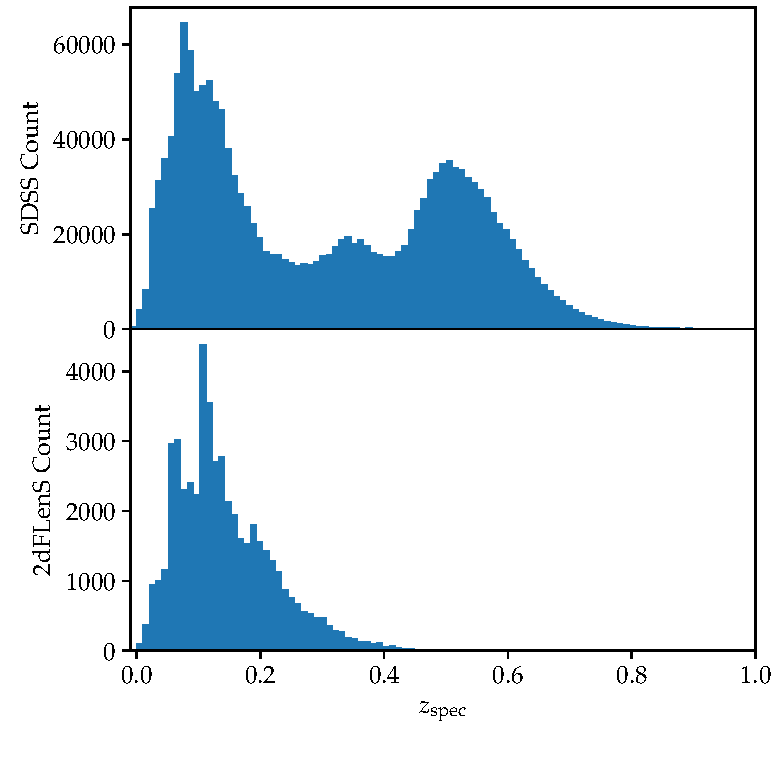
\includegraphics[width=0.9\textwidth]{zpec_hist.pdf}
    \caption{Histogram of objects in SDSS and 2dFLenS by spectroscopic redshift.}
    \label{fig:spec_hist}
  \end{figure}

  \jn{define photometry}

  \section{Colours}

  \jn{write about the 5 magnitudes used}

  \jn{plot the filters}

  \jn{why these 5 filters?}

  \jn{getting canonical colours from the five filters}

  \section{Datasets}
  \jn{TODO: WRITE}

  \subsection{SDSS}
  The spectroscopic redshift distribution of objects in SDSS is presented in \cref{fig:spec_hist}.

  \jn{TODO: WRITE}

  \subsection{2dfLenS}
  The spectroscopic redshift distribution of objects in 2dfLenS is presented in \cref{fig:spec_hist}.

\chapter{Regression on Photometric Redshifts}

Let $\cX \subset \bbR^d$ be bounded. Let $f$ map $\cX$ to $\bbR$. Regression is the task of reconstructing such an $f$ from finitely many examples of its inputs and outputs.

We are given a set \[
  \cD = \left\{\left(\bx_1, y_1\right), \dots, \left(\bx_n, y_n\right)\right\}
\] of $n$ samples of $f$, where $y_1, \dots, y_n$ are the \textit{labels}. Let $\cP$ be the probability distribution of the label noise. Then for all $i$, \[
  y_i = f(\bx_i) + \epsilon \text{ for some error } \epsilon \sim \cP \text{.}
\]

Let $\hat\cF$ be our space of possible approximations; its exact membership depends on our model. We want to find $\hat f \in \hat\cF$ that is the best approximation of $f$. Each candidate approximation $\hat f_c \in \hat\cF$ can be assigned a likelihood that quantifies how good an approximation it is:\[
    p\left(\hat f_c \;\middle|\; \cD \right) \text{.}
\] We define $\hat f$ to be the function that maximises this likelihood:\[
    \hat f \coloneqq \argmax_{\hat f_c \in \cF} p\left(\hat f_c \;\middle|\; \cD \right) \text{.}
\] The definition of this likelihood is dependent on our assumptions, such as on our assumed noise distribution $\cP$ and on any assumptions we have about $f$.

In our specific case we will always assume that the noise is distributed according to a Gaussian with a mean of $0$ and a variance $\sigma^2$ that we leave as a hyperparameter\footnote{A hyperparameter is a parameter that depends on the distribution of our data.}.

We apply regression to find objects' redshifts from their photometric measurements, as a cheaper alternative to spectroscopy. We are given a set of example objects' photometric measurements and spectoscopic redshifts, and we wish to predict the redshift of any new object whose photometric colours have been measured. Hence, in our case $\cX \subset \bbR^5$ is the space of photometric measurements.

Let $f : \cX \to \bbR$ be the physical function that maps photometric measurements to redshifts. It is not obvious why it is valid to assume that such a function exists. Indeed, it is physically possible to have two objects with the same photometry, but different redshifts. We can let $f$ be the function that maps photometric measurements to to any corresponding object's most likely redshift. This lets us treat any inconsistency as any other source of noise.

Some models are capable of not only predicting $f$ but also returning a measure of its confidence in its prediction. Gaussian Process regression is an example of such a model. This measure of confidence becomes crucial when we seek to improve our predictions with active learning.

\section{Assessing performance}

To assess the performance of our model, we must have a way of quantifying its accuracy. We withhold a portion of our data into a testing set $\cD'$ of $n'$ elements such that \[
  \cD' = \{(\bx'_1, y'_1), \dots, (\bx'_{n'}, y'_{n'})\}
\] and $\cD$ is disjoint from $\cD'$.

For each testing sample $(\bx'_i, y'_i)$, define the prediction as\[
  \hat y'_i \coloneqq \hat f(\bx'_i)
\] and define the $\delta$ error as \[
  \delta_i \coloneqq y'_i - \hat y'_i\text.
\] For redshifts, define $dz$ as \[
  dz_i \coloneqq \frac{\delta_i}{1 + y'_i} \text.
\]

For a perfect predictor then,\[
  \hat y'_i = y'_i \text{ for all }i=1, \dots, n'\text{,}
\] so $\delta_i = 0$. Unfortunately, perfect predictors are rarely possible to produce. This is due to noise in the labels, and also because of our inherent ability to reconstruct an arbitrary function from a finite number of samples.

Hence, we must assign a numerical score to each predictor, so we can compare their performance. The fraction of variance unexplained is a commonly used score. Others, more specific to photometric redshifts, are the mean $dz$ error, the $dz$ deviation, and the fraction of $dz$ outliers. Photometric redshifts suffer from a high number of outliers, which do not have as much an influence on these redshift-specific scores.

\subsection{Fraction of Variance Unexplained}
The fraction of variance unexplained (FVU) measures the fraction of the variance of the labels $y'_1, \dots, y'_{n'}$ not explained by the predictor. For a predictor that explains the entire variance $\mathrm{FVU}=0$, and for a predictor that explains none of the variance $\mathrm{FVU}=1$.

Let $\mathrm{VAR_{err}} \coloneqq \frac{1}{n'}\sum_{i=1}^{n'}\delta_i^2$ be the mean squared $\delta$ error. If the mean $\delta$ error is zero, this equals the variance\footnote{For a finite set $S = \{s_1, \dots, s_{\abs{S}}\} \subset \bbR$ of $\abs{S}$ elements, we define the variance as $\var S \coloneqq \frac1{\abs{S}}\sum_{i=1}^{\abs{S}}(s_i - \overline{s})^2$, where $\overline{s} \coloneqq \frac1{\abs{S}}\sum_{i=1}^{\abs{S}}s_i$ is the mean of $S$.} of the $\delta$ errors. Let $\mathrm{VAR_{tot}} \coloneqq \var\{y'_1, \dots, y'_{n'}\}$ be the variance of the labels of the testing set. Note that $\mathrm{VAR_{err}}$ varies with the predictor, whereas $\mathrm{VAR_{tot}}$ is constant for each testing set. We define \[
  \mathrm{FVU} \coloneqq \frac{\mathrm{VAR_{err}}}{\mathrm{VAR_{tot}}} \text{.}
\]  Values of $\mathrm{FVU}$ closer to $0$ are better.

Intuitively, a perfect predictor explains the entire variance of the labels, so we expect it to yield $\mathrm{FVU} = 0$. Indeed, a perfect predictor has $\delta_1 = \dots = \delta_{n'} = 0$, so $\mathrm{VAR_{err}} = 0$, implying that $\mathrm{FVU} = 0$.

For a predictor that always returns the mean of the testing set, $\mathrm{VAR_{err}} = \mathrm{VAR_{tot}}$ by definition, so $\mathrm{FVU} = 1$, as expected since a predictor that always returns the mean explains none of the variance. A predictor with $\mathrm{FVU} > 1$ then performs worse by our metric than a predictor that always returns the mean.

\subsection{Mean $dz$ error}

The mean $dz$ error is specific to photometric redshifts. It is defined as \[
  \textrm{mean $dz$ error} \coloneqq \frac{1}{n'}\sum_{i=1}^{n'} \abs{dz_i} \text.
\] Values closer to $0$ are better.

The $dz$ error scales the $\delta$ error to account for the magnitude of the label, since an error of $0.5$ on a label of $0.1$ is relatively more significant than an error of $0.5$ on a label of $1$. It does so by dividing the error by $1 + y'_i$, noting that the minimum possible redshift is $-1$.

Unlike the fraction of variance unexplained error, the mean $dz$ error depends on a sum of absolute errors, as opposed to the sum of squared errors. This is an important distinction, as the sum of squared errors is more likely to be overly influenced by outliers.

\subsection{$dz$ bias}

The $dz$ bias is also specific to photometric redshifts. It quantifies whether the predictor is more likely to over- or underestimate the redshift. It is defined as\[
  \textrm{$dz$ bias} \coloneqq \frac{1}{n'}\sum_{i=1}^{n'} dz_i \text.
\] Note that unlike the FVU and the mean $dz$ error, the $dz$ bias is permitted to be negative. In addition, a $dz$ bias of zero, whilst desirable, does not indicate a perfect predictor.

\subsection{$dz$ deviation}

The $dz$ deviation is defined as the half-width of redshift deviation $dz$ containing $68.3\%$ of all objects. More formally, the $dz$ deviation is the smallest $\sigma \in \bbR_{\geq0}$ such that $68.3\%$ of $dz_i$ errors are within $[-\sigma, \sigma]$. It has the advantage of completely discarding outliers beyond percentile $68.3$, vastly reducing their influence.

\subsection{Fraction of $dz$ outliers}

The fraction of $dz$ outliers is defined as the fraction of objects with $\abs{dz} > 0.1$. It quantifies the fraction of objects whose redshifts fail to be explained by the model.

\section{Existing methods}

\jn{write intro to section}

\jn{cite Chris' paper heavily}

\subsection{Kernel density estimation}

\jn{Write about Chris's KDE}

\subsection{Neural networks}

\jn{write}

\subsection{Boosted decision trees}

\jn{Boosted decision trees}

\subsection{Template methods}

\jn{write}

\section{Linear Regression}

  \begin{wrapfigure}{R}{0.4\textwidth}
    \centering
    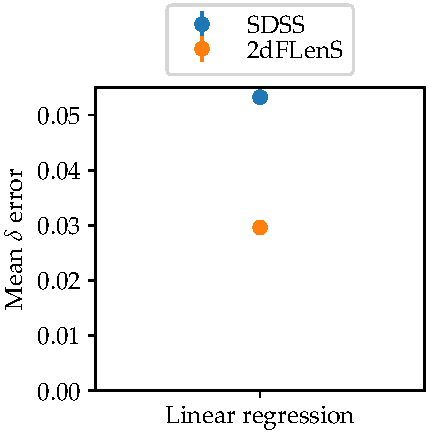
\includegraphics[width=0.4\textwidth]{linreg_plain.pdf}
    \caption{Error of linear regression with linear features. Lower is better; error of $0$ means perfect fit. Note that since this regression is purely linear, a bias term is not used.}
    \label{fig:linreg_plain}
  \end{wrapfigure}

  \begin{wrapfigure}{R}{0.4\textwidth}
    \centering
    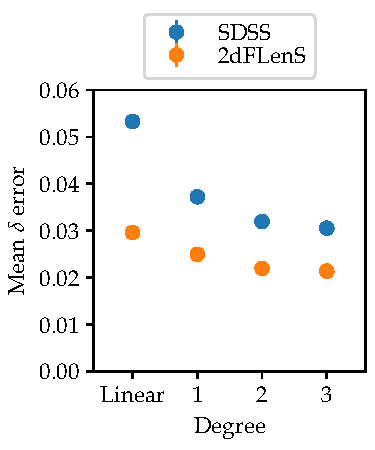
\includegraphics[width=0.4\textwidth]{linreg_polynomial.pdf}
    \caption{Error of linear regression with polynomial features. Note that degree 1 polynomial features are equivalent to linear regression with a bias term.}
    \label{fig:linreg_polynomial}
  \end{wrapfigure}

Linear regression is the simplest regression model. \jn{is it?}

Choose $m \in \bbN$. Choose $\phi_1, \dots, \phi_m$, each mapping $\cX$ to $\bbR$.

We make the assumption that $\hat f$ is a linear combination of $\phi_1, \dots, \phi_m$. Then \[
    \hat f(\bx) = \bphi(\bx)^\top \bw \text{,}
\] where we define \[
    \bphi(\bx) \coloneqq \begin{bmatrix} \phi_1(\bx) \\ \vdots \\ \phi_n(\bx) \end{bmatrix}\text{,}
\] and where $\bw \in \bbR^m$ is the weights vector we wish to find.

Define also\[
    \Phi \coloneqq \begin{bmatrix}
        \bphi(\bx_1)^\top \\
        \vdots \\
        \bphi(\bx_m)^\top
    \end{bmatrix} \text{.}
\]

We also make the assumption that $p(\by \mid \hat f, X)$ depends only on how well $\hat f$ approximates $f$ at $x_1, \dots, x_n$. More formally, defining \[
    \hat y_i \coloneqq f(\bx_i) \text{ for }i = 1, \dots, n\text{ and }
    \hat\by \coloneqq \begin{bmatrix} \hat y_1 \\ \vdots \\ \hat y_n \end{bmatrix} \text{,}
\] we have that
\begin{align}
    p(\by \mid \hat f, X) &= \prod_{i = 1}^{n} \cN\left(\hat y_i \;\middle|\; y_i, \sigma^2\right) \label{eq:linearlikelihood} \\
    &= \prod_{i = 1}^{n} \frac{1}{\sqrt{2\pi\sigma^2}} \exp\left(-\frac{\left(\hat y_i - y_i\right)^2}{2\sigma^2}\right) \text. \nonumber
\end{align} We wish to find $\bw$ that maximises this likelihood. This is equivalent to minimising the negative log likelihood,\begin{align*}
    -\log p(\by \mid \hat f, X) &= - \log \prod_{i = 1}^{n} \frac{1}{\sqrt{2\pi\sigma^2}} \exp\left(-\frac{\left(\hat y_i - y_i\right)^2}{2\sigma^2}\right) \\
    &= - \sum_{i = 1}^{n} \log\left(\frac{1}{\sqrt{2\pi\sigma^2}} \exp\left(-\frac{\left(\hat y_i - y_i\right)^2}{2\sigma^2}\right)\right) \\
    &= - \sum_{i = 1}^{n} \left(\log\frac{1}{\sqrt{2\pi\sigma^2}} + \log\exp\left(-\frac{\left(\hat y_i - y_i\right)^2}{2\sigma^2}\right)\right) \\
    &= - \sum_{i = 1}^{n} \left(-\frac{1}{2}\log\left(2\pi\sigma^2\right) -\frac{\left(\hat y_i - y_i\right)^2}{2\sigma^2}\right) \\
    &=  \frac{n}{2}\log\left(2\pi\sigma^2\right) + \frac{1}{2\sigma^2}\sum_{i = 1}^{n}\left(\hat y_i - y_i\right)^2 \text{.}
\end{align*} Since $\frac{n}{2}\log(2\pi\sigma^2)$ is a constant, minimising $-\log p(\by \mid \hat f, X)$ is equivalent to minimising $\frac{1}{2\sigma^2}\sum_{i = 1}^{n}(\hat y_i - y_i)^2$. Further, since $1/\sigma^2$ is constant, this is equivalent to minimising $\frac12\sum_{i = 1}^{n}(\hat y_i - y_i)^2$.

We call this our loss function and write\[
    E(\bw) = \frac12\sum_{i = 1}^{n}(\hat y_i(\bw) - y_i)^2 \text{.}
\] Note that we can compute it without knowing $\sigma^2$. For reasons that should be clear, this is called the \textit{sum of squares} error.

The optimal weights vector is then given by \[
    \argmax_{\bw} p(\by \mid \hat f(\bw), X) = \argmin_{\bw} E(\bw) \text{.}
\]

We can solve this analytically. We first note that \begin{align*}
    E(\bw) &= \frac12\sum_{i = 1}^{n}(\bphi(\bx_i)^\top \bw - y_i)^2 \\
    &= \frac12\sum_{i = 1}^{n}(\Phi \bw - \by)_i^2 \\
    &= \frac12(\Phi \bw - \by)^\top(\Phi \bw - \by) \text{.}
\end{align*} Setting the derivative to zero to find the minimum, \[
    \frac{dE(\bw)}{d\bw} = \Phi^\top (\Phi\bw - \by) = \mathbf{0} \text{.}
\] Solving, the minimum is \[
    \bw  = \left(\Phi^\top\Phi\right)^{-1}\Phi^\top\by
\]

\subsubsection{Feature differences}

We show that create new features that are pairwise differences between existing features does not affect a linear model since the same predictor can be found using the original features.

Consider a dataset with $n$ features. Let $\mathbf{x}$ be the $n$-dimensional feature vector.

Let $\mathbf{D}$ be an $n \times n$ matrix such that \[
    \mathbf{D}_{ij} \coloneqq \mathbf{x}_i - \mathbf{x}_j \text{.}
\]

Let $\bm{\alpha}$ be an $n$-dimensional weights vector for $\mathbf{x}$ and let $\mathcal{B}$ be an $n \times n$ weights matrix for $\mathbf{D}$. Let our predictor be\[
    y = \bm{\alpha} \cdot \mathbf{x} + \langle \mathcal{B}, \mathbf{D} \rangle_F \text{,}\label{eq:pred1}\tag{$*$}
\] where $\langle \mathcal{B}, \mathbf{D} \rangle_F$ is a Frobenius inner product.

Let $\hat{\bm{\alpha}}$ be an $n$-dimensional vector such that \[
    \hat{\bm{\alpha}}_i \coloneqq \bm{\alpha}_i + \sum_{j=1}^n \mathcal{B}_{ij} - \sum_{j=1}^n \mathcal{B}_{ji} \text{.}
\] We show that a predictor defined as \[
    y = \hat{\bm{\alpha}} \cdot \mathbf{x}
\] is equivalent to \eqref{eq:pred1}.

We have that\begin{align*}
    \hat{\bm{\alpha}} \cdot \mathbf{x} &= \sum_{i=1}^n \mathbf{x}_i\left( \bm{\alpha}_i + \sum_{j=1}^n \mathcal{B}_{ij} - \sum_{j=1}^n \mathcal{B}_{ji} \right) \\
    &= \sum_{i=1}^n \mathbf{x}_i\bm{\alpha}_i +  \sum_{i=1}^n \sum_{j=1}^n \mathbf{x}_i \mathcal{B}_{ij} - \sum_{i=1}^n \sum_{j=1}^n \mathbf{x}_i \mathcal{B}_{ji} \\
    &= \sum_{i=1}^n \mathbf{x}_i\bm{\alpha}_i +  \sum_{i=1}^n \sum_{j=1}^n \mathbf{x}_i \mathcal{B}_{ij} - \sum_{i=1}^n \sum_{j=1}^n \mathbf{x}_j \mathcal{B}_{ij} \\
    &= \bm{\alpha}\cdot\mathbf{x} +  \sum_{i=1}^n \sum_{j=1}^n \mathcal{B}_{ij} \left(\mathbf{x}_i - \mathbf{x}_j \right) \\
    &= \bm{\alpha}\cdot\mathbf{x} + \langle \mathcal{B}, \mathbf{D} \rangle_F
\end{align*} as desired.

Note that this does not apply to non-linear models where a nonlinear transformation is applied to $\mathbf{D}$. It also does not necessarily hold when regularisation is applied to the weights.

\section{Kernels}

A kernel is a function $k : \bbR^d \times \bbR^d \to \bbR$ such that \[
    k(\bx, \bx') = \langle \bvarphi\left(\bx\right), \bvarphi\left(\bx'\right)\rangle \text{,}
\] where $\bvarphi : \bbR^d \to H$ maps our feature space $\bbR^d$ to a real Hilbert space $H$. Intuitively then, we can think of a kernel as an inner product in a different space.

Like other inner products, a kernel can be thought of as a similarity measure. For example, $k(\bx, \bx') = 0$, then $\bx$ and $\bx'$ are orthogonal in $H$, and thus not similar at all by our definition.

Kernels permit us to generalise our earlier basis transformations $\bphi : \bbR^d \to \bbR^m$ to $\bvarphi : \bbR^d \to H$. Due to the possibly infinite-dimensional nature of $H$, we cannot use $\bvarphi$ directly. Instead, we can take advantage of it by computing $k$.

\subsection{Examples of Kernels}
\subsubsection{Gaussian Kernel}

  \begin{wrapfigure}{R}{0.4\textwidth}
    \centering
    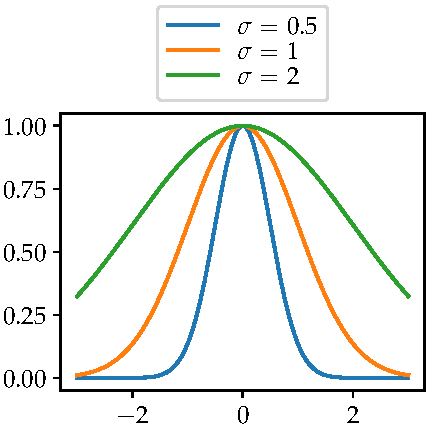
\includegraphics[width=0.4\textwidth]{gaussian_kernel_plot.pdf}
    \caption{$K(0, x)$, where $K$ is the Gaussian kernel.}
    \label{fig:gaussian_kernel}
  \end{wrapfigure}

The Gaussian Kernel is defined by \[
    k(\bx, \bx') \coloneqq \exp\left( - \frac{\norm{\bx - \bx'}^2}{2\sigma^2} \right) \text{,}
\] where the hyperparamerer $\sigma$ is known as the \textit{length scale}. This is visualised in \cref{fig:gaussian_kernel}.

An alternative definition involves length scales $\sigma_1, \dots, \sigma_d$, permitting us to set the length independently for each axis. The definition is \[
    k(\bx, \bx') \coloneqq \exp\left( - \frac{1}{2}\left(\bx - \bx'\right)^T\Sigma^{-1}\left(\bx - \bx'\right) \right) \text{,}
\] where \[
    \Sigma = \begin{bmatrix}
        \sigma_1^2 & & \makebox(0,0){\text{\huge0}} \\
        & \ddots & \\
        \mbox{\huge 0} & & \sigma_d^2
    \end{bmatrix} \text{.}
\]

\subsubsection{Rational-Quadratic Kernel}

  \begin{wrapfigure}{R}{0.4\textwidth}
    \centering
    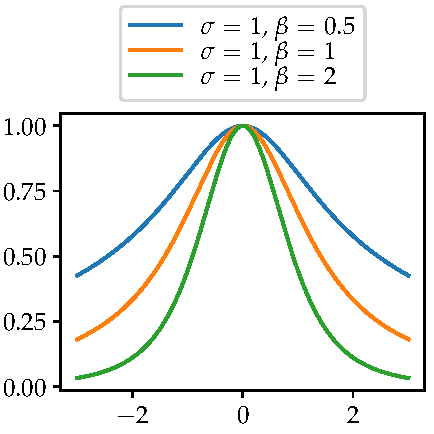
\includegraphics[width=0.4\textwidth]{rational_quadratic_kernel_plot.pdf}
    \caption{$K(0, x)$, where $K$ is the Rational-Quadratic kernel.}
    \label{fig:rational_quadratic_kernel}
  \end{wrapfigure}

The Rational-Quadratic Kernel is defined by \[
    k(\bx, \bx') \coloneqq \left(1 + \frac{1}{2\gamma}\norm{\bx - \bx'}^2\right)^{-\beta} \text{,}
\] where $\gamma > 0$ is the \textit{length scale} and $\beta > 0$ is the \textit{shape parameter}. It can be thought of as an infinite sum of gaussian kernels.

The Rational-Quadratick Kernel is visualised in \cref{fig:rational_quadratic_kernel}.

Setting $\gamma = \beta \gamma_0$ and letting limiting $\beta \to \infty$ yields a Gaussian kernel with length scale $\gamma_0$.

\subsubsection{Exponential Kernel}
  \begin{wrapfigure}{R}{0.4\textwidth}
    \centering
    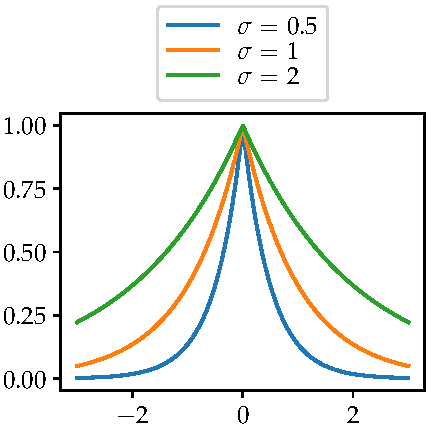
\includegraphics[width=0.4\textwidth]{exponential_kernel_plot.pdf}
    \caption{$K(0, x)$, where $K$ is the Exponential kernel.}
    \label{fig:exponential_kernel}
  \end{wrapfigure}

  The exponential is defined by \[
    k(\bx, \bx') \coloneqq \exp\left( - \frac{\norm{\bx - \bx'}}{\sigma} \right) \text{,}
  \] where $\gamma > 0$ is the \textit{length scale} and $\beta > 0$ is the \textit{shape parameter}. It is plotted in \cref{fig:exponential_kernel}.


\subsubsection{Mat\'ern Kernel}

  \begin{wrapfigure}{R}{0.4\textwidth}
    \centering
    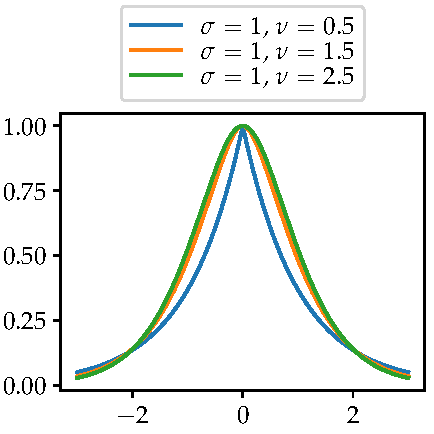
\includegraphics[width=0.4\textwidth]{matern_kernel_plot.pdf}
    \caption{$K(0, x)$, where $K$ is the Mat\'ern kernel.}
    \label{fig:matern_kernel}
  \end{wrapfigure}

For some $\bx$ and $\bx'$, define $d \coloneqq \norm{\bx - \bx'}$. The Mat\'ern Kernel is defined by \[
    k(\bx, \bx') \coloneqq \frac{2^{1-\nu}}{\Gamma(\nu)}\left(\frac{\sqrt{2\nu}d}{\sigma}\right)^\nu K_\nu\left(\frac{\sqrt{2\nu}d}{\sigma}\right)
\]$K_\nu$ is the modified Bessel function of the second kind, $\Gamma$ is the Gamma function, $\nu$ is positive parameter, and $\ell$ is the length scale. It is differentiable $\floor{\nu-1}$ times. See \cref{fig:matern_kernel} for a visualisation.

For some values of $\nu$ it can be simplified. When $\nu = 1/2$,
 \[
   k(\bx, \bx') = \exp\left(-\frac{d}{\sigma}\right) \text{;}
 \] when $\nu=3/2$, \[
   k(\bx, \bx') = \left(1 + \frac{\sqrt{3}d}{\sigma}\right)\exp\left(-\frac{\sqrt{3}d}{\sigma}\right) \text{;}
 \] and when $\nu = 5/2$,\[
  k(\bx, \bx') = \left(1 + \frac{\sqrt{5}d}{\sigma} + \frac{5d^2}{3\sigma^2}\right)\exp\left(-\frac{\sqrt{5}d}{\sigma}\right) \text.
 \] Observe that for $\nu=1/2$, it simplifies to the exponential kernel. The other two simplifications are an exponential kernel multiplied by a polynomial in $d/\sigma$.
\subsection{Kernel Approximations}

For large dataset, computing $K$ becomes expensive as has a space complexity of $O(n^2)$.

\subsubsection{RBF Sampling}

RBF Sampling approximates the Gaussian Kernel by sampling from its Fourier transform. \jn{I literally don't know if this is correct}

\jn{prove}

\subsubsection{Empirical Kernel Map}

\jn{TODO: WRITE}


\subsection{Kernelised Linear Regression}

  \begin{wrapfigure}{R}{0.4\textwidth}
    \centering
    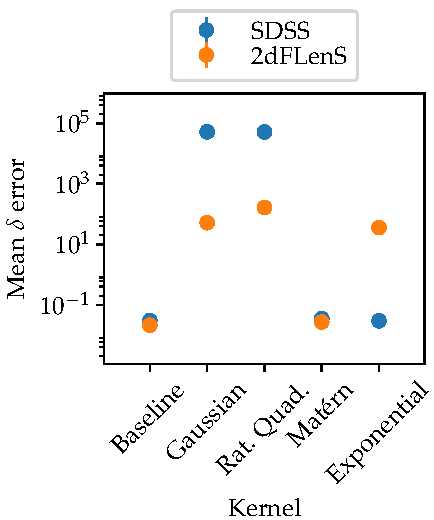
\includegraphics[width=0.4\textwidth]{linreg_kernelised.pdf}
    \caption{Error of kernelised linear regression. The $\sigma$ is the median distance between training $\bx$ values.}
    \label{fig:linreg_kernelised}
  \end{wrapfigure}

Consider the problem of regression. We are given a function $f : \bbR^d \to \bbR$ for some $d \in \bbN$. We are also given $n$ points $\bx_1, \dots, \bx_n$ for which we know the values. In other words, we know $y_1, \dots, y_n$ where \[
    y_i \coloneqq f(\bx_i)\text{ for }i = 1, \dots, n\text{.}
\]

Let $\phi : \bbR^d \to \bbR^r$ be the feature map. If we are performing linear regression, then we want to find $\bw \in \bbR^r$ such that \[
    f(\bx) \approx \phi(\bx)^T \bw \text{.}
\]

Define \[
    \Phi \coloneqq \begin{bmatrix}
        \phi(\bx_1)^T \\
        \vdots \\
        \phi(\bx_n)^T \\
    \end{bmatrix} \text{ and }\by \coloneqq \begin{bmatrix}
        y_1 \\
        \vdots \\
        y_n
    \end{bmatrix} \text{.}
\]

We wish to use the least-squares error with $\ell_2$ regularisation. We can define the error function to be $E : \bbR^r \to [0, \infty)$ such that \[
    E(\bw) \coloneqq \frac{1}{2}\norm{\by - \Phi\bw}_2^2 + \frac{\lambda}{2} \norm{\bw}_2^2 \text{,}
\] where $\lambda > 0$ is the regularisation constant.

We know that $\bw \in \spn\{\phi(\bx_1), \dots, \phi(\bx_n)\}$. Hence, there exists $\bv \in \bbR^n$ such that \[
    \bw = \Phi^T\bv \text{.}
\]

We can rewrite the error function as $E : \bbR^n \to [0, \infty)$ such that \[
    E(\bv) = \frac{1}{2}\norm{\by - \Phi\Phi^T\bv}_2^2 + \frac{\lambda}{2} \norm{\Phi^T\bv}_2^2 \text{.}
\] Letting $K \coloneqq \Phi\Phi^T$ be the kernel matrix,\[
    E(\bv) = \frac{1}{2}\norm{\by - K\bv}_2^2 + \frac{\lambda}{2} \bv^T K \bv \text{.}
\] Then $k(\bx, \bx') \coloneqq \phi(\bx) \cdot \phi(\bx')$ is our kernel function.

Differentiating, we find \begin{align*}
    E'(\bv) &= -K^T(\by - K\bv) + \frac{\lambda}{2} (K + K^T)\bv \\
    &= K(K\bv - \by) + \lambda K\bv \text{,}
\end{align*} since $K$ is symmetric. The minimum exists at $E'(\bv) = 0$. Simplifying, we find,\[
    K(K + \lambda I)\bv = K\by \text{.}
\] There may be multiple solutions. One solution is at \[
    \bv = (K + \lambda I)^{-1}\by \text{.}
\]

For a given input $\bx$, the prediction is then \begin{align*}
    f(\bx) &\approx \phi(\bx)^T \bw \\
    &= \phi(\bx)^T \Phi \bv \\
    &= \phi(\bx)^T \Phi (K + \lambda I)^{-1}\by \\
    &= K_* (K + \lambda I)^{-1}\by \text{,}
\end{align*} where we define \[
    K_* \coloneqq \phi(\bx)^T \Phi \text{.}
\]

This is very similar to Gaussian Process regression, where the prediction is \[
    f(\bx) = K_*\left(K + \sigma^2 I\right)^{-1}\by \text{.}
\]

Kernelised linear regression is then equivalent to Gaussian Process regression when $\lambda = \sigma^2$.

\section{Regularisation}

  \begin{wrapfigure}{R}{0.4\textwidth}
    \centering
    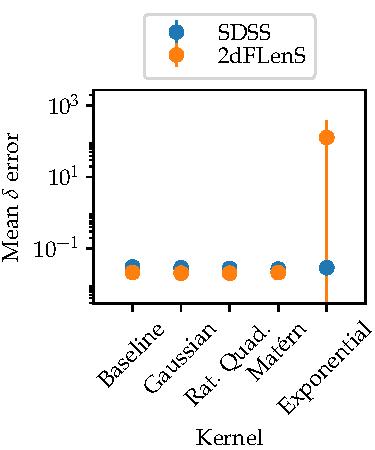
\includegraphics[width=0.4\textwidth]{linreg_kernelised_regularised.pdf}
    \caption{Error of regularised kernelised linear regression. The regularisation constant $\lambda$ is $0.001$.}
    \label{fig:linreg_kernelised_regularised}
  \end{wrapfigure}

Often we wish to limit the complexity of $\hat f$ to prevent overfitting. We can make the assumption that every element of the weights vector $\bw$ is likely to be close to zero: \[
    p(w_i) = \cN(w_i \mid 0, \mu)
\] for some variance $\mu > 0$.

We can then change the likelihood in \cref{eq:linearlikelihood} to account for this: \begin{align*}
    p(\by \mid \hat f, X) &= \prod_{i = 1}^{n} \cN\left(\hat y_i \;\middle|\; y_i, \sigma^2\right) \label{eq:linearlikelihood} \prod_{i = 1}^{m}\cN(w_i \mid 0, \mu) \\
    &= \prod_{i = 1}^{n} \frac{1}{\sqrt{2\pi\sigma^2}} \exp\left(-\frac{\left(\hat y_i - y_i\right)^2}{2\sigma^2}\right) \prod_{i = 1}^{m}\frac{1}{\sqrt{2\pi\mu}} \exp\left(-\frac{w_i^2}{2\mu}\right) \text{.}
\end{align*}

Computing the negative log likelihood,\[
    -\log p(\by \mid \hat f, X) = \frac{n}{2}\log\left(2\pi\sigma^2\right) + \frac{1}{2\sigma^2}\sum_{i=1}^{n}\left(\hat y_i - y_i\right)^2 + \frac{m}{2}\log\left(2\pi\mu\right) + \frac{1}{2\mu}\sum_{i=1}^{m}w_i^2 \text{.}
\]

Eliminating the constant terms, we find that \begin{align*}
    \argmin_{\bw} - \log p\left(\by \;\middle|\; \hat f, X\right) &= \argmin_{\bw} \left(\frac{1}{2\sigma^2}\sum_{i=1}^{n}\left(\hat y_i - y_i\right)^2 + \frac{1}{2\mu}\sum_{i=1}^{m}w_i^2\right) \\
    &= \argmin_{\bw} \frac{1}{\sigma^2}\left(\frac12\sum_{i=1}^{n}\left(\hat y_i - y_i\right)^2 + \frac{\lambda}{2}\sum_{i=1}^{m}w_i^2\right) \text{,}
\end{align*} where we defined $\lambda \coloneqq \sigma^2 / \mu > 0$. Eliminating the positive multiplicative constant,\begin{align*}
    \argmin_{\bw} - \log p\left(\by \;\middle|\; \hat f, X\right) &= \argmin_{\bw} \left(\frac12\sum
    _{i=1}^{n}\left(\hat y_i - y_i\right)^2 + \frac{\lambda}{2}\sum_{i=1}^{m}w_i^2\right) \\
    &= \argmin_{\bw} \left(\frac12\left(\hat \by - \by\right)^\top\left(\hat \by - \by\right) + \frac{\lambda}{2}\bw^\top\bw\right) \\
    &= \argmin_{\bw} \left(\frac12\left(\Phi \bw - \by\right)^\top\left(\Phi \bw - \by\right) + \frac{\lambda}{2}\bw^\top\bw\right) \text.
\end{align*}

Our loss now depends on $\bw$ and $\lambda$ and is given by \[
    E(\bw, \lambda) = \frac12\left(\Phi \bw - \by\right)^\top\left(\Phi \bw - \by\right) + \frac{\lambda}{2}\bw^\top\bw \text{,}
\] where $\lambda$ is our \textit{regularisation constant}: a higher value implies a simpler model, reducing the likelihood of overfitting, but increasing the chance of underfitting.

We can find $\bw$ that minimises the loss. Taking the derivative and setting it to $\mathbf{0}$,\[
    \frac{dE(\bw, \lambda)}{d\bw} = \Phi^\top(\Phi\bw - \by) + \lambda \bw = \mathbf{0} \text{.}
\] Solving,\[
    \bw = \left(\Phi^\top\Phi + \lambda I\right)^{-1}\Phi^\top\by \text.
\]

\section{Finding Hyperparameters}

  \subsection{Grid Search}

  Grid Search is one technique that permits us to find hyperparameters. We must first define a finite set of candidate hyperparameter configurations $H$.

  The algorithm is as follows:
  \begin{minted}[
    gobble=4,
    linenos,
    fontsize=\small,
    frame=lines,
    python3=true
  ]{python}
    def cross_validate(H, train_X, train_y, validation_X, validation_y)
        best_parameters = None
        best_score = float('-inf')

        for h in H:
            regressor.set_params(**h)
            regressor.train(train_X, train_y)
            score = regressor.score(validation_X, validation_y)

            if score > best_score:
                best_parameters = h

        return best_parameters
  \end{minted}

  The technique is called grid search since $H$ is often a cartesian product of the options for each hyperparameter.

  \subsection{Bayesian Optimisation}
  Our Gaussian Process Regression has six hyperparameters: a length scale for each of the five features and a regularisation constant. The high dimensionality of the hyperparameter space makes it difficult to find the optimal parameters using grid search. Bayesian optimisation may be used instead to speed up this process.

\jn{derive bayesian optimisation}

\subsection{Automatic Relevance Determination}
  \begin{figure}
    \centering
    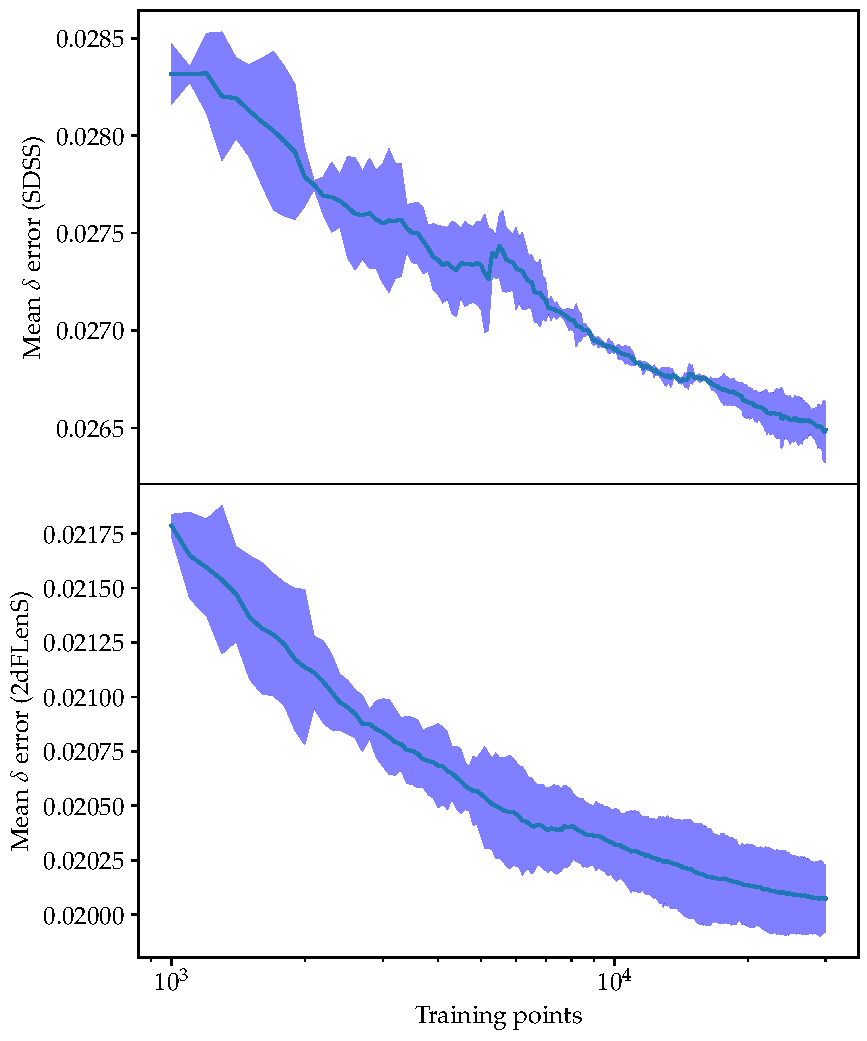
\includegraphics[width=0.9\textwidth]{passive_delta.pdf}
    \caption{Passive learning curve: Mean $\delta$ error plotted against the number of training points for both SDSS and 2dFLenS. The training points are chosen at random. The shaded interval represents the two-sigma confidence interval.}
    \label{fig:passive_delta}
  \end{figure}

  \begin{figure}
    \centering
    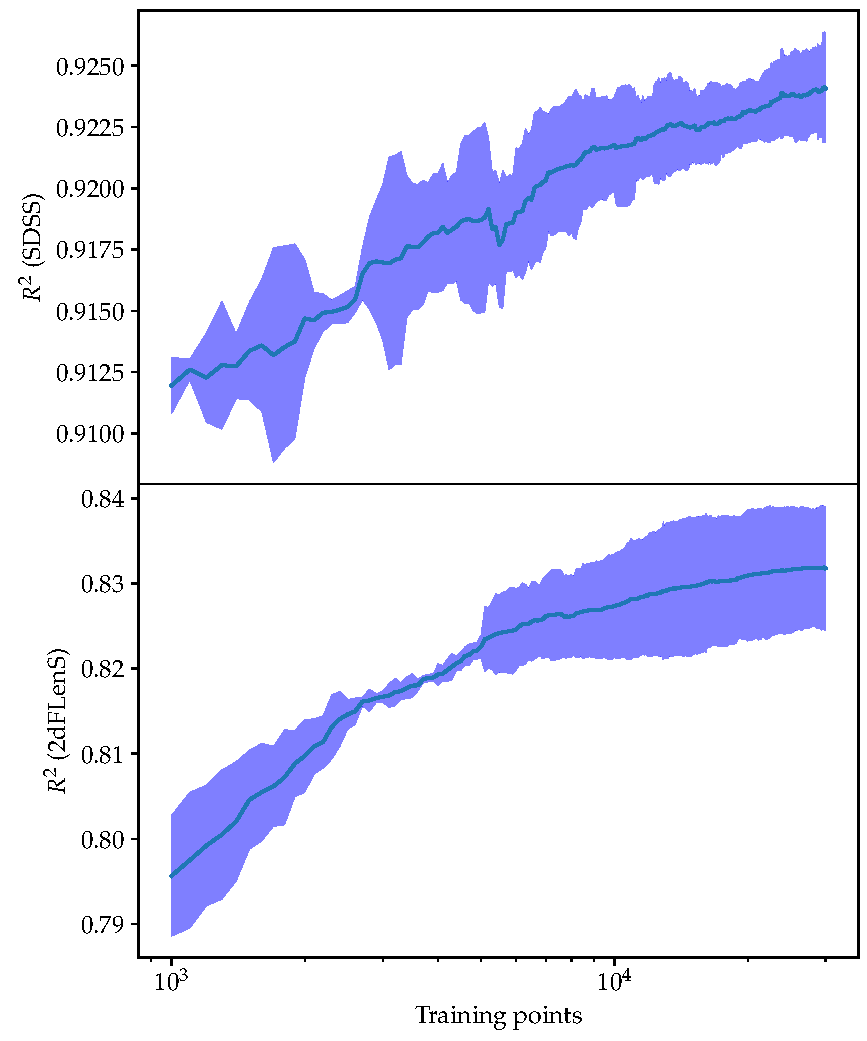
\includegraphics[width=0.9\textwidth]{passive_r2.pdf}
    caption{Passive learning curve: $R^2$ error plotted against the number of training points for both SDSS and 2dFLenS. The training points are chosen at random. The shaded interval represents the two-sigma confidence interval.}
    \label{fig:passive_r2}
  \end{figure}

Automatic Relevance Determination is another technique that may be used to find the hyperparameters for our Gaussian Process Regression.

Consider the problem of linear regression. We have a five-dimensional feature space $\cX$. The features have \jn{noise vairances?} variances $\lambda_1, \dots, \lambda_5$, respectively. We place a prior on our regression weights.

Our prior variance for each weight is proportional to the variance of the weight. We also assume that the weights are uncorrelated. Hence, our sum-of-squares loss function becomes \jn{how?}\[
    \frac12\norm{X\bw - \by}^2 + \alpha \bw^T \Lambda \bw \text.
\]

\jn{now talk about that weird convergence bullshit for the regularisation constant}

\jn{we don't care about pruning right? because we're not pruning...}

\section{Gaussian Processes}
Consider the task of reconstructing a function $f: \bbR^d \to y$ from finitely many samples. As a complication, each target sample contains is noisy, with the noise having a variance $\sigma^2$.

More formally, we are given a finite set of tuples\[
    \{ (\vec{x_1}, y_1), \dots, (\vec{x_n}, y_n) \}\text,
\] where \[
    y_i \sim \cN\left(f(\vec{x_i}), \sigma^2\right)\text.
\] We wish to be able to predict $f(\vec{x})$, given an arbitrary $\vec{x}$.

A Gaussian process is a distribution over functions. Formally, a Gaussian process is defined as a `collection of random variables, any finite number of which have a joint Gaussian distribution.'\footnote{C. E. Rasmussen \& C. K. I. Williams, Gaussian Processes for Machine Learning, the MIT Press, 2006, ISBN 026218253X.}

Defining \begin{align*}
    m(\vec{x}) &\coloneqq \bbE[f(\vec{x})] \text, \\
    k(\vec{x}, \vec{x}') &\coloneqq \bbE[(f(\vec{x}) - m(\vec{x}))(f(\vec{x'}) - m(\vec{x'}))],
\end{align*} we write \[
    f(\vec{x}) \sim \cG\cP(m(\vec{x}), k(\vec{x}, \vec{x'}))\text.
\]

We write \begin{align*}
    \vec y &\coloneqq (y_1, \dots, y_n)^\intercal \text, \\
    X &\coloneqq (\vec{x_1}, \dots, \vec{x_n})^\intercal \text, \\
    K(X, X) &\coloneqq \begin{bmatrix}
        k(\vec{x_1}, \vec{x_1}) & \cdots & k(\vec{x_1}, \vec{x_n}) \\
        \vdots & \ddots & \vdots \\
        k(\vec{x_n}, \vec{x_1}) & \cdots & k(\vec{x_n}, \vec{x_n})
    \end{bmatrix}\text.
\end{align*}

Then $\cov(\vec{y}) = K(X, X) + \sigma_n^2I$.

Let $\vec{f_*}$ be the test predictions and $X_*$ be the test inputs. Under the prior, we have that the joint distribution of the observed targets and of the function values at the test locations is \[
    \begin{bmatrix}
        \vec{y} \\ \vec{f_*}
    \end{bmatrix} \sim \cN\left(\vec0, \begin{bmatrix}
        K(X, X) + \sigma_n^2I & K(X, X_*) \\
        K(X_*, X) & K(X_*, X_*)
    \end{bmatrix}\right)\text.
\]

It can then be derived that \[
    \vec{f_*} \mid X, \vec{y}, X_* \sim \cN\left(\overline{\vec{f_*}}, \cov(\vec{f_*})\right)\text,
\] where \[
    \overline{\vec{f_*}} = K(X_*, X)[K(X, X) + \sigma_n^2I]^{-1}\vec{y}\text,
\] and \[
    \cov(\vec{f_*}) = K(X_*, X_*) - K(X_*, X)[K(X, X) + \sigma_n^2I]^{-1}K(X, X_*)\text.
\]

The value for $\vec{f_*}$ that has the highest probability is the mean of the Gaussian from which it is sampled. Hence, we can predict that \begin{equation}
    \label{eq:pred}
    \vec{f_*} \approx K(X_*, X)[K(X, X) + \sigma_n^2I]^{-1}\vec{y}\text,
\end{equation} with the variance for each element of the vector being\[
    \var(\vec{f_*}_i) = \left( K(X_*, X_*) - K(X_*, X)[K(X, X) + \sigma_n^2I]^{-1}K(X, X_*) \right)_{ii}\text.
\]

One can observe from \cref{eq:pred} that the prediction is a linear combination of the observations $\vec{y}$. This is in contrast to linear regression, where the prediction is a linear combination of the inputs.

\subsection{Equivalence to Kernelised Linear Regression}

Observe that \cref{eq:pred} the equation for kernelised linear regression with regularisation. Thus, Gaussian Process regression and kernelised regular regression always return the same expected value, although kernelised linear regression is unable to estimate the variance of that prediction.

\section{Approximating Gaussian Processes}

Gaussian Process regression relies on our calculation of $(K+\sigma_n^2)^{-1}$, which has a high time complexity\footnote{$O(n^3)$ for a naive implementation; $O(n^{2.373})$ for an optimised method based on the Coppersmith–Winograd algorithm.\jn{reference}}. This obviously does not scale well to large training sets. Instad, we can approximate Gaussian Process Regression with algorithms of a lower time complexity.

\subsection{My Favourite Approximation}

\jn{wtf is it called}

We can approximate this matrix product with a complexity that is linear in $n$.

Let $\Phi \in \bbR^{n \times f}$ for $f \ll n$ be our kernel approximation for the training set. Then $K \approx \Phi \Phi^T$. Let $\phi \in \bbR^{f}$ be the kernel approximation for the value we wish to predict for. Then $K_* \approx \Phi \phi$. Hence,\begin{align*}
    K_*^T(K+\sigma_n^2)^{-1}K_* &\approx \phi^T\Phi^T  \left(\Phi \Phi^T + \sigma_n^2I\right)^{-1} \Phi\phi \\
    &= \phi^T\Phi^T  \left( \sigma_n^{-2}I - \sigma_n^{-2}\Phi(\sigma_n^{2} + \Phi^T\Phi)^{-1}\Phi^T\right) \Phi\phi \\
    &=  \sigma_n^{-2}\phi^T\Phi^T\Phi\phi - \sigma_n^{-2}\phi^T\Phi^T \Phi(\sigma_n^{2} + \Phi^T\Phi)^{-1}\phi\Phi^T\Phi
\end{align*}

Then \[
    \hat f(\bx) = \sigma_n^{-2} \phi^T\Phi^T\by - \sigma_n^{-2} \phi^T\Phi^T\Phi(\sigma_n^{2} + \Phi^T\Phi)^{-1}\Phi^T\by
\] and \[
    \var \hat f(\bx) = \phi^T\phi - \sigma_n^{-2}\Phi^T \phi^T\phi\Phi - \sigma_n^{-2}\Phi^T \phi^T\Phi(\sigma_n^{2} + \Phi^T\Phi)^{-1}\Phi^T\phi\Phi\text.
\]

Numerical instabilities present difficulties for small $\sigma_n^2$ as the matrix $(\Phi\Phi^T + \sigma_n^2I)$ becomes closer to being singular.

\subsection{Linear Regression and KDE}

The mean of Gaussian Process Regression can also be approximated by linear regression. Letting $\Phi$ be the kernel approximation on the training set, we find that the regression weights are\[
    \bw = \left(\Phi^\top\Phi + \sigma_n^2 I\right) \Phi^\top\by\text,
\] where $\sigma_n^2$ becomes the regularisation constant. This can be computed in $O(nf)$ time by solving the linear equation instead of directly performing the matrix inversion.

It remains to find an approximation to the variance predicted by Gaussian Process regression. Kernel density estimation can be used to approximate this. Let $D$ be the density estimator. Then we expect $\left(D(\bx)\right)^1$ and $\var f(\bx)$ to have a monotonic relationship.

The actual relationship could probably be found by regression on the estimated densities and the estimated variances of an artificially generated dataset.

This method is less prone to numerical instabilities than my favourite approximation. However it was not used in this work, as a more direct approximation was available.


\chapter{Active Learning}

\jn{define active learning}

\jn{motivate}

\section{Recommenders}

In active learning, a recommender is a function that prioritises some unlabelled training samples over others. \jn{rewrite?} It can be thought of in two equivalent ways.

A recommender can be thought of as a function $\pi : \cP(\cX) \times \bbN \to \cP(\cX)$. Then $\pi(P, r)$ returns $r$ of its most preferred samples from the sample pool $P$.

A recommender can also be a function $\varpi : \cX \to \bbR$. Then $\varpi(\bx)$ returns the preference score it assigns to $\bx$, with a higher score being more preferred.

Given a recommender $\varpi : \cX \to \bbR$ returning a score, we can define a recommender $\pi : \cP(\cX) \times \bbN \to \cP(\cX)$ returning a set of samples. To obtain $\pi(P, r)$ by choose the top $r$ samples from $P$ as scored by $\varpi$.

Similarly, given a recommender $\pi : \cP(\cX) \times \bbN \to \cP(\cX)$, we can define a recommender $\varpi : \cX \to \bbR$ returning a score. \jn{TODO: finish}



\section{Measuring performance}

\subsection{Learning curves}
A learning curve tracks the performance of a model with a given recommender. Let $T = \{t_1, \dots, t_r\} \subset \bbN$ with $t_1 < \dots < t_r$ be the counts of training points that we try. Then the learning curve is a function $\ell : T \to \bbR_{\geq0}$, whose output is an error.

For a recommender $\pi$ and a model $F : \cP(\cX \times \cY) \to \cF$, we generate the learning curve $\ell$ with \cref{alg:generate-learning-curve}. Intuitively, we begin by training $F$ with $t_1$ random samples and measuring its performance. We then repeatedly add points recommended by $\pi$, train the model, and measure its performance. This gives us $F$'s performance as a function of the cardinality of the training.

We can qualitatively describe the performance of a recommender by examining the learning curve it generates. In general, the better the accuracy of $F$ trained on points given by $\pi$, the better $\pi$ is.

An example of a learning curve can be seen in figure \jn{BLAH}. In that figure, the uncertainty recommender clearly outperforms the passive (random) recommender.

\begin{algorithm}[H]
    \KwData{
      \\\quad A recommender $\pi$,
      \\\quad A function $F : \cP(\cX \times \cY) \to \cF$ generating a predictor from training samples,
      \\\quad A function $e : \cF \to \bbR_{\geq0}$ yielding the error of a predictor,
      \\\quad A training sample pool $P \subseteq \cX$,
      \\\quad Labels for samples in $P$,
      \\\quad Training example counts to try $T = \{t_1, \dots, t_r\} \subset \bbN$ with $t_1 < \dots < t_r$.
    }
    \KwResult{A learning curve $\ell : T \to \bbR_{\geq0}$.}

    $\textrm{labelled} \leftarrow t_1$ training samples from $P$ with labels $y$, random without replacement

    $\hat f \leftarrow F(\textrm{labelled})$

    $\ell(t_1) \leftarrow e(\hat f)$

    \For{$i \in 2, \dots, r$}{
      $\textrm{chosen} \leftarrow t_i - t_{i-1}$ training samples from $P \setminus \textrm{labelled}$ chosen by $\pi(\hat f)$

      $\textrm{labelled} \leftarrow \textrm{labelled} \cup \textrm{chosen}$ with labels

      $\hat f \leftarrow F(\textrm{labelled})$

      $\ell(t_i) \leftarrow e(\hat f)$
    }
    \caption{Generating a learning curve.}
    \label{alg:generate-learning-curve}
\end{algorithm}

\subsection{Deficiency}

\jn{todo: define $\fF$ as the set of possible models}

\jn{todo: define $\fD$ as the set of possible training sets}

\jn{todo: define $\cE$ as the set of possible error functions}

\jn{todo: define $\cT$ as the set of possible counts}

The deficiency $d$ is a function $d : \fD \times \fF \times \cE \times \cT \times \Pi \to \bbR$. Intuitively, $d(P, F, e, T, \pi)$ measures the room for improvement that a recommender $\pi \in \Pi$ has on a model $F \in \fF$, a training set pool $P \in \fD$, at times $T \in \cT$, according to an error function $e \in \cE$. In general, the lower the deficiency, the better $\pi$ performs on our predictor and dataset.

\jn{todo: consider defining as $d$ as $\cL \times \cT \to \bbR$, where $\cL$ is the set of possible learning curves}

To define $d(P, F, e, T, \pi)$, let $\ell : T \to \bbR_{\geq0}$ be the learning curve with a predictor $F$, a recommender $\pi$, a candidate pool $P$, and an error function $e$ and $F$ at times $T = \{t_1, \dots, t_r\}$ ordered in ascending order. Generally, $\ell$ reach its minimum at $t_r$. This is because, in general, models perform better with more training samples; hence, training on all available samples is likely to yield the best possible model. We use $\ell(t_r)$ as a baseline for a `perfect' recommender.

\jn{todo: write about impossibility of perfect recommender}

\jn{a recommender may or may not be perfect depending on testing set}

\jn{even a perfect recommender will not reach deficiency $0$}

Then we define $d$ to be the signed area between $\ell$ and the line $y = \ell(t_r)$. \jn{justify use of trapezoidal as opposed to just integrating} We compute it by applying the trapezoidal rule: \begin{align*}
  d(\pi; P, F, e, T) &= \sum_{i=1}^{r-1} (t_{i+1} - t_i)\left(\frac12\ell(t_i) + \frac12\ell(t_{i+1}) - \ell(t_r)\right) \text.
  \\&\text{\jn{make more readable. justify the subtraction of $\ell(t_r)$}}
\end{align*}

Observe that the deficiency is permitted to be negative. This may occur if $F$ trained on the entirety of $P$ performs worse than $F$ trained on a subset of $P$ with size $t_i$ chosen by $\pi$. Then $\ell(t_i) - \ell(t_r)$ is negative, so we cannot place a lower bound on the integral. \jn{reword. this is shite}

\jn{make plot to visualise}

\jn{TODO: change all $T$ sets to $\bt$ vectors}

For a fixed, $P$, $F$, $e$, and $\bt$, we may compute the deficiencies of recommenders $\pi$ and $\pi'$ to compare them. Let $\ell$ and $\ell'$ be the learning curves of $\pi$ and $\pi'$ respectively. Then $\ell(t_r) = \ell'(t_r)$, since each trains $F$ on the entire pool $P$ at time $t_r$.\footnote{Whilst this is true mathematically, in reality $\ell(t_r)$ and $\ell'(t_r)$ are approximately but not exactly equal due to numerical inaccuracies. To permit the deficiencies to be compared directly, we find the average of the individual baselines and use it to compute the deficiencies.} Then $d(\pi;\dots)$ and $d(\pi';\dots)$ measure the area between $\ell$ and $\ell'$ respectively and a common baseline. \jn{this doesn't make sense. edit plz} Hence, it is possible to directly compare the deficiencies to rank the recommenders.



\section{Possible recommenders}

\subsection{Passive}

\jn{TODO: consider calling it a `random' recommender and relating to passive learning}

The passive recommender is the baseline upon which we wish to improve. It yields random samples from the candidate pool. This makes it equivalent to adding extra training points without utilising any active learning techniques. The passive learning curves we use as a baseline are shown in figures \jn{BLAH}, \jn{BLAH}, and \jn{BLAH}. We use these to assess the performance of our active learning techniques.

\subsection{Uncertainty}
  \begin{figure}
    \centering
    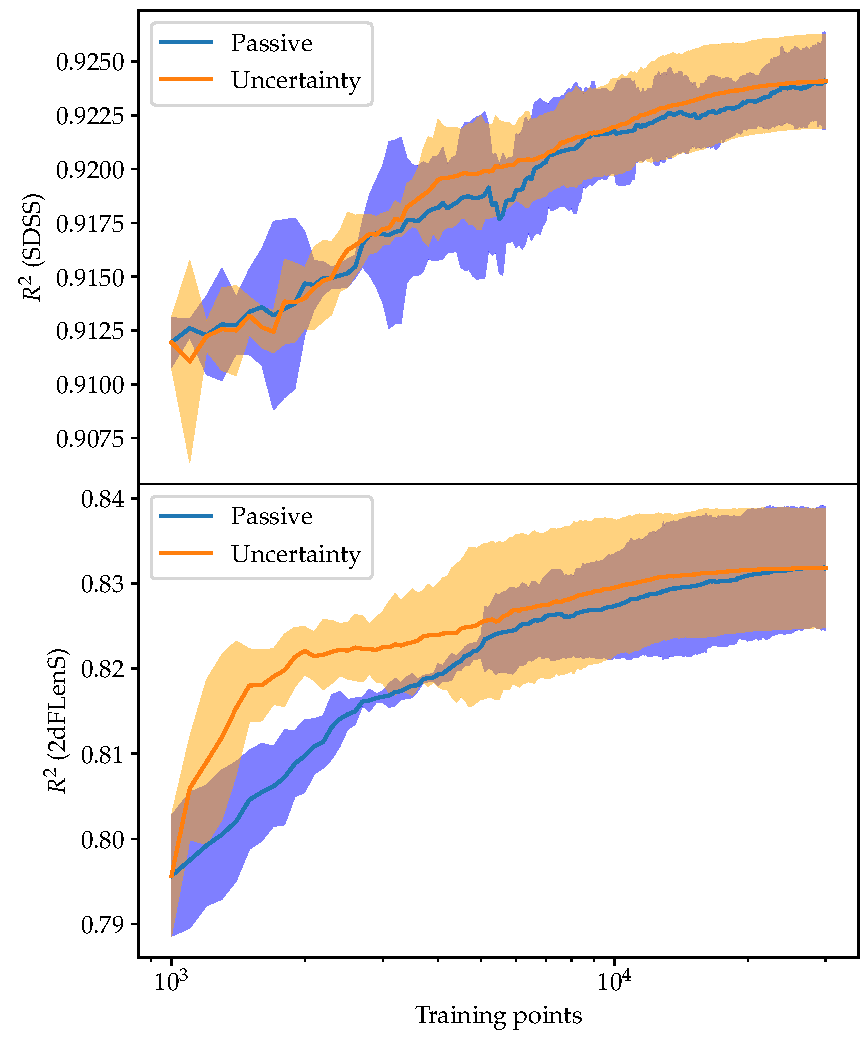
\includegraphics[width=0.9\textwidth]{uncertainty_r2.pdf}
    \caption{Learning curve: $R^2$ error plotted against the number of training points for both SDSS and 2dFLenS. The training points are chosen either at random (Passive) or using uncertainty recommendation with a batch size of $100$. The shaded interval represents the two-sigma confidence interval.}
    \label{fig:uncertainty_r2}
  \end{figure}

Let $\var \hat f$ be the variance returned by Gaussian PRocess Regression. The uncertainty recommender is defined as \[
    \argmax_{c \in \cC} \var\hat f(c) \text.
\]

Intuitively, it returns the points that we are the most uncertain about. If we are uncertain about a point, then we have less information about that particular area of the feature space. Hence the points that we are uncertain about would be good additions to the training set.

This intuition fails at the start of our training. This is because we end up focusing on points that we are very unsure about, which tend to be on the long tail of the distribution. Since, in our case, the distribution is five-dimensional, this is a very poor strategy, as we spread out our efforts and neglect the core of the distribution.

\jn{learning curve}

\subsection{Density}

Let $\cD : \cX \to \bbR^+$ be a density function for the dataset. This can be derived from the training set by fitting a gaussian mixture model or by Kernel Density Estimation. The recommended points are \[
    \argmax_{c \in \cC} \cD(c) \text.
\]

\jn{learning curve on pure density}

As seen above, this recommendation strategy yields good results at the start of the learning curve, when we have trained on very few datapoints. However, late on the curve flattens out and no longer produces very good results, being overtaken by uncertainty recommendation.

\subsection{Boltzmann sampling}

Consider a physical system that occupies one of $M$ possible states. Let $T > 0$ be the temperature of the system. For each $i=1, \dots, M$, the state $s_i$ has potential energy $\varepsilon_i$. If $\varepsilon_i < \varepsilon_{i'}$, then we must input energy equalling $\varepsilon_{i'} - \varepsilon_i$ to move from the state $s_i$ to $s_{i'}$. As an example, consider a hydrogen atom consisting of a nucleus and an electron. The electron occupies one of two shells around the nucleus: the inner shell or the outer shell. Energy is required to move this electron the inner shell to the outer shell; hence, the state of lying in the outer shell is of higher energy.

\jn{lily: `A system seeks to minimise its energy, resulting in a non-uniform probability of states. Higher-energy states are rarely sampled, but introducing kinetic energy in the form of higher temperatures can increase their likelihood. The probability of a state then depends on its energy and the temperature T of the system, formalised in the Boltzmann distribution:'}

The probability of the system existing in a particular state is not uniform. \jn{unclear, reword} A system seeks to minimise its energy, so the lower-energy states are more likely. However, higher-energy states are not impossible, particularly in high temperatures: a sufficiently hot gas will become ionised, entering a higher-energy state. The probability of a state $s_i$ then depends on its energy $\varepsilon_i$ and on the temperature $T$ of the system. It follows the \textit{Boltzmann distribution}:\[
  p(s_i) = Z\exp\left(\frac{-\varepsilon_i}{k_\mathrm{B}T}\right) \text,
\] where $k_\mathrm{B}$ is the Boltzmann constant, and $Z \coloneqq 1/\sum^{M}_{i=1}\frac{-\varepsilon_i}{k_\mathrm{B}T}$ ensures that the probabilities sum to $1$.

We can apply these physical principles to active learning to obtain a wider variety of recommendations. Since many scoring functions are continuous, any two recommended samples are likely to be correlated, yielding redundant information. Boltzmann sampling helps reduce this effect.

Let $\varpi : \cX \to \bbR$ be a recommender that assigns a score to the candidate samples. Let $P = \{\bx_1, \dots, \bx_N\}$ be the pool of candidates; think of each as a state. Then the energy of $\bx_i$ is $\varepsilon_i = -\varpi(\bx_i)$ since we prefer higher scores. A Boltzmann sampler with temperature $T$ then recommends a sample $\bx_i$ with probability \[
  p(\bx_i) \propto \exp\left(\frac{-\varepsilon_i}{T}\right) \text{\footnotemark}.
\]\footnotetext{Observe that this formula omits the Boltzmann constant for simplicity.} Observe that samples with higher scores are still preferred. The strength of that preference is inversely proportional to $T$.

\jn{learning curves of boltzmann on uncertainty and density with different temperatures}

\subsection{Mixing recommenders}

From the plots above, we see that different recommenders excel at different stages of the training. Density recommendation is best when we are starting off, and uncertainty recommendation helps us tackle the long tail of the distribution in the later stages. The need to combine the benefits of both strategies becomes clear.

There are two ways of combining recommenders, depending on their definition.

If we think of a recommender as a function that assigns a score to a candidate, and we are given two recommenders $A : \cC \to \bbR$ and $B : \cC \to \bbR$, then we can derive a third recommender $C : \cC \to \bbR$ as \[
    C(c) \coloneqq kA(c) + lB(c)
\] for come $k, l \in \bbR$.

This is not always the most helpful strategy. The distribution of scores returned by $A$ and $B$ could be totally different, in which case it doesn't make sense to scale each by a constant and sum them. They need to be on the same order and on the same scale.

Instead, another way of deriving a mixed recommender is to think about probabilities. When selecting $n$ elements from $C$, we want to select elements from $A$ with probability $p$ and elements from $B$ with probability $1-p$. Hence, we can combine $pn$ elements from $A$ and $(1-p)n$ elements from $B$ to form the $n$ elements from $C$.

A constant $p$ (or equivalently constant $k$ and $l$) with combine both the advantages and disadvantages of each strategy, yielding a mediocre recommender. We know, however, that uncertainty recommendation and density recommendation excel at different stages of training. It makes sense to prioritise density recommendation at the start, and uncertainty recommendation towards the end.

This is reminiscent of the problem of exploration vs exploitation. Uncertainty scores are mostly noise until we have enough data in our training set.

\jn{figure out optimal function for p/kl}

\jn{helpful plot}

\bibliography{references}{}
\bibliographystyle{plain}

\end{document}
